\documentclass[12pt, a4paper]{article} % Document font size and paper size
\usepackage[utf8]{inputenc}
\usepackage{DejaVuSans}
\usepackage{graphicx}
\usepackage{epstopdf}
\usepackage{multicol}
\usepackage{color}
\usepackage{framed}
\usepackage[usenames,dvipsnames,svgnames,table]{xcolor}
\usepackage{hyperref}
\usepackage{geometry} % Allows the configuration of document margins
\usepackage{color}
\usepackage{listings}
\usepackage[T1]{fontenc}
\usepackage{eurosym}

\usepackage{titlesec}

%\usepackage[protrusion=true,expansion=true]{microtype} % Better typography

\definecolor{orange}{HTML}{FF9900}
\definecolor{shadecolor}{RGB}{150,150,150}
  
\graphicspath{ {./images/} }

\geometry{a4paper, textwidth=6.5in, textheight=8in, marginparsep=6pt, marginparwidth=.6in} % Document margin settings

\lstset{literate=%
    {Ö}{{\"O}}1
    {Ä}{{\"A}}1
    {Ü}{{\"U}}1
    {ß}{{\ss}}2
    {ü}{{\"u}}1
    {ä}{{\"a}}1
    {ö}{{\"o}}1
}

\hypersetup{
 pdfauthor={Schumilin, Tseyzer},
 pdftitle={Seminararbeit}
 pdfsubject={Seminararbeit},
 pdfkeywords={Not set}
}

\hyphenation{
wirt-schaft-liche
wissen-schaft-liche 
Wäh-rend
Un-ter-nehm-en
Fin-anz-ver-wal-tung
Wiss-en-schaft-ler
durch-zu-führ-en
in-ge-nieur-wis-sen-schaft-lich
Ver-öf-fent-lich-un-gen
}

\renewcommand{\figurename}{Abbildung} 
\renewcommand{\tablename}{Tabelle} 
\newcommand{\specialcell}[2][c]{%
  \begin{tabular}[#1]{@{}c@{}}#2\end{tabular}}

\renewcommand*{\familydefault}{\sfdefault}



\titleformat{\section}
{\color{orange}\normalfont\LARGE\bfseries}
{\color{orange}\thesection}{1em}{}
[
\vspace{0.5ex}%
\rule{\textwidth}{2pt}
\vspace{2ex}%
] % after-code

\titleformat{\subsection}
{\color{orange}\normalfont\large\bfseries}
{\color{orange}\thesubsection}{1em}{}

\titleformat{\subsubsection}
{\color{orange}\normalfont\normalsize\bfseries}
{\color{orange}\thesubsubsection}{1em}{}
\begin{document}

%%%%%%%%%%%%%%%%%%%%%%%%%
% TITEL
%%%%%%%%%%%%%%%%%%%%%%%%%
\thispagestyle{empty}

\begin{titlepage}
%%\let\footnotesize\small \let\footnoterule\relax
\begin{center}

\hbox{}
\vskip 1.8cm


\includegraphics[width=0.6\textwidth]{./logo}~

\hbox{}
\vfill
\vskip 1cm
Business Plan\\
von\\[2mm]
\vskip 1cm

{\large\bfseries Artem Schumilin \& Igor Tseyzer\\}
\vskip 4cm
{\bfseries Seminar}\\
Developing Business Models \\
for the Semantic Web (WS 13/14) \\
%Universität Karlsruhe (TH)\\[2ex]
\vskip 2cm

\vskip 1cm
Januar 2014

\end{center}
\vfill
\end{titlepage}

%%%%%%%%%%%%%%%%%%%%%%%%%
% CONTENT
%%%%%%%%%%%%%%%%%%%%%%%%%

\tableofcontents
\newpage

%%%%%%%%%%%%%%%%%%%%%%%%%
% Executive Summary Artem und Igor
%%%%%%%%%%%%%%%%%%%%%%%%%
\section{Zusammenfassung}

SemLit ist ein präzise und zuverlässige Web-Dienstleistung, die für Informationssuche in Bereich Informatik entwickelt. Auf Basis von semantische Quellenindexierung erlaubt SemLit real-time Suche in Informationquellen, Informationsabfrageverwaltung und benachbarte Informationsquellensuche.\\
Die Zielgruppe ist vor allem Studenten und Wissenschaftler in Bereich der  Ingenieurwesen und Technologie, Technische Hochschulen und Unternehmen.
Das Projekt wurde von zwei Studenten von Karlsruher Institut für Technologie gegründet. Das Team hast entsprechende Kenntnisse in Bereichen von Web Technologien, Semantic Technologien, Softwareentwicklung sowie Unternehemens- und Finanzverwaltung. \\
Auf der Basis von Finanzplanung und Entwicklungsstrategie lasst sich das Break-Even Punkt am 17. Monat der Unternehmenstätigkeit erwarten. Die Entwicklung bis Break-Even dient dafür eine gut funktionierte Infrastruktur zubauen, die als Grundstein der Erfolg dient. Die Chancen und Risiken Analyse zeigt, dass die Finanzsituation nach Break-Evan eine gute Aufsicht auf weitere erfolgreiche Entwicklung hat. Die geplante Umsatz nach 24 Monate umfasst ca. 40 000 Euro pro Monat.\\
Die genutzte Technologie könnte leicht am verwandte Bereiche eingesetzt werden, wie zum Beispiel Informationssuche und Verwaltung in wirtschaftliche und juristische Bereichen. Das beschriebene Einsatz kann sehr leicht durchgeführt werden, dank schon existierende Infrastruktur und Technologie.\\
SemLit hat sehr gute Aufsicht auf Markterfolg und könnte als effektive Investition berücksichtigen werden. 



\newpage

%%%%%%%%%%%%%%%%%%%%%%%%%
% Geschäftsidee Artem
%%%%%%%%%%%%%%%%%%%%%%%%%
\section{Geschäftsidee}


\subsection{Worum es hier geht}
Eine Studie von International Data Corporation (IDC, eines der führenden Marktforschungs-unternehmen in der IT-Industrie) aus dem Jahr 2005\footnote[1]{\textit{White Paper on Hidden Cost of Information Work}, IDC, 2005.} hat gezeigt, dass ein Wissensarbeiter im Durchschnitt rund ein Viertel seiner Arbeitszeit alleine auf die Informationssuche aufwendet. In der wissenschaftlichen Forschung ist dieser Anteil unseren Schätzungen zufolge noch größer. Gesucht wird dabei vor allem nach Information in Form von wissenschaftlichen Publikationen. Weil Publikationen im Idealfall den Stand der Technik abbilden, ist deren Studium ein Grundpfeiler erfolgreicher wissenschaftlicher Praxis. 

\begin{table}[h!]
  \centering
  \begin{large}
	\begin{itshape}
  \begin{tabular}{c}\hline
	\\
  {\color{orange}„Wenn ich weiter geblickt habe, so deshalb,} \\ 
	{\color{orange}weil ich auf den Schultern von Riesen stehe.“} \\
	{\hfill \color{orange}\textit{Isaac Newton, 1676} } \\
	\\\hline
  \end{tabular}
	\end{itshape}
  \end{large}
\end{table}

Neben den obligatorischen Veröffentlichungen in Journals und Konferenzbändern bergen Blogs und Magazine häufig eine nicht minder wichtige Quelle für neue Ideen und Herangehensweisen. An dieser Stelle kommen allerdings vier wichtige Faktoren ins Spiel, die eine erfolgreiche Literaturrecherche erheblich erschweren: 

\begin{description}
  \item[\textbf{\color{orange}{Informationsuniversum wächst:}}] \hfill \\
  Die Zahl möglicher Quellen und potentiell wertvoller Informations-Items wächst rasant: 
In 2008 erschienen allein in den neun\footnote[2]{Nach UNESCO Science Report 2010: GER, FRA, UK, RUS, JPN, KOR, CHN, CAN, USA} großen Wissenschaftsnationen 760.671 Veröffentlichungen. Bei der gegenwärtigen jährlichen Wachstumsrate von 3,26\% wird sich diese Zahl in zwanzig Jahren verdoppeln. 
  \item[\textbf{\color{orange}{Information veraltet:}}] \hfill \\
  Neu produziertes Wissen veraltet heute schneller als jemals zuvor. Neue Entwicklungen in einem Forschungsfeld werden schnell entdeckt, aufgegriffen und weiterentwickelt. Wenn man Fortschritt erzielen möchte, ist jede Verzögerung bei der Informationssuche ein schwerwiegender Nachteil. 
  \item[\textbf{\color{orange}{Wissensgebiete werden vernetzt:}}] \hfill \\
  Die Grenzen zwischen den Disziplinen verschwimmen zunehmend. Bahnbrechende Arbeiten über Datenverarbeitung werden manchmal in Biologie-Journals publiziert, weil beispielsweise die Genomforschung ohne Informatik nicht mehr auskommt. Solche potentiell interessanten Informations-Events bleiben natürlich unentdeckt, wenn man die Aufmerksamkeit unmittelbar auf das eigene Feld beschränkt. 
 \item[\textbf{\color{orange}{Verfügbare Such-Tools sind unzulänglich:}}] \hfill \\
	Die Möglichkeiten der Suche in der globalen Informationswolke, bereitgestellt durch Incumbents wie Google und Microsoft, sind weitgehend auf Schlüselworte beschränkt. Dabei ist die Suche nach Bedeutungs-Nuancen und Konzepten das, was eine effektive Literaturrechere ausmacht. 
\end{description} Diese Probleme wird \textsc{\color{orange}{SemLit}} lösen. Mit semantischen Technologien werden wir die Praxis der Literaturarbeit umkrempeln. Im Folgenden beschreiben wir, wie das im Detail geschehen soll. 

\begin{table}[h!]
  \centering
  \begin{large}
	\begin{itshape}
  \begin{tabular}{c}\hline
  \\
  {\color{orange}Ein Wissensarbeiter verbringt durchschnittlich }\\
  {\color{orange}24\% seiner Zeit mit Informationssuche.}\\
  \\\hline
  \end{tabular}
	\end{itshape}
  \end{large}
\end{table}


%=======================================

\subsection{Know-how Träger}
Die Idee und Umsetzung wird von zwei Studenten des Karlsruher Instituts für Technologie (KIT) entwickelt. {\color{orange}Artem Schumilin} studiert Wirtschaftsingenieurwesen (M.Sc) und {\color{orange}Igor Tseyzer} studiert Informationswirtschaft (B.Sc). Während des Studiums am KIT haben beide Gründer die notwendigen Kenntnisse in Web- und Semantic-Web-Technologien gesammelt, was als stabiles Fundament für den Aufbau und weitere Entwicklung der Firma dienen soll. 
\begin{figure}[h!]
\centering
\includegraphics[width=0.6\textwidth]{jsi-aifb-logo}
\end{figure}
\emph{<hier: Liste relevanter Fähigkeiten und Erfahrungen>}
Igor wird im neuen Unternehmen die Marketingstrategie entwickeln und den Vertrieb organisieren, während Artem Verantwortung für die Produktentwicklung und die Finanzen übernehmen wird. 
\\
\\
Neben dem KIT-eigenen Gründernetzwerk stehen den Gründern renommierte Partner aus der Forschung zur Seite: 
Das Josef-Stefan-Institut (JSI) hat mit \emph{Enrycher} die weltweit führende \emph{named entity recognition engine} entwickelt und tritt damit als der Tchnologiepartner von SemLit auf. 
Das Institut AIFB des KIT erweist sich als erfahrener Mentor in Sachen Ausgründung im Bereich semantischer Technologie und wird das Start-Up mit seinen Kontakten und Rat unterstützen.

%=======================================

\subsection{Innovation}

\textsc{Schritt 0:} wo es beginnt\\
Wir beginnen bei den Informations-Items, die im Internet zur freien Verfügung stehen. Dazu gehören vor allem die Abstracts von wissenschaftlichen Veröffentlichungen aus Journals und Konferenzbänden aber auch Artikel in relevanten Blogs und Online-Magazinen. Die Vielzahl der Quellen wird automatish überwacht, um die Nahezu-Echtzeit-Anforderung erfüllen zu können.\\
{\color{orange}Unsere Kunden können die Auswahl der Quellen auf ihre individuellen Bedürfnisse anpassen. }
\\
\\
\textsc{Schritt 1:} die Semantik hinter dem Text\\
Der Kerngedanke hinter SemLit gründet auf den Möglichkeiten, die durch semantische Repräsentation von Textinformation entehen. Dazu gehört die Erkennung von named entities und ihrer Beziehungen untereinander. Mit JSI's Enrycher steht uns die derzeit weltbeste Technologie bereit, mit deren Hilfe wir die Extraktion semantischer Information aus Textdokumenten realisieren. 
\\
\begin{figure}[h!]
\centering
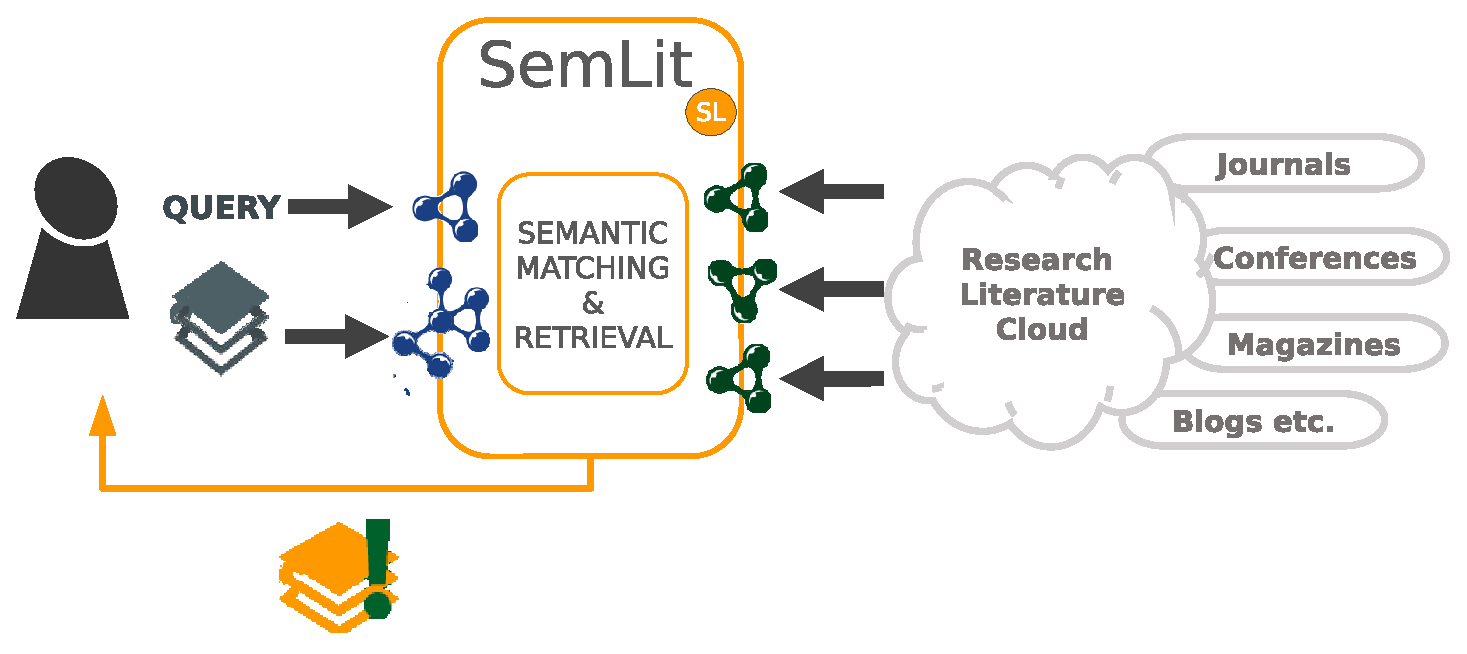
\includegraphics[width=0.9\textwidth]{idea}
\caption{Funktionsschema von SemLit}
\label{fig:idea}
\end{figure}
\\
\textsc{Schritt 2: Informationswunsch äußern}\\
Wie die Textinformation auf der einen Seite, können auf der anderen Seite auch die Suchanfragen der Kunden semantisch repräsentiert werden. Damit kann der Benutzer extrem nuancierte Konzepte ausdrücken. 
Dieses semantische \emph{information retrieval} liefert deutlich bessere Ergebnisse als die gewöhnliche Schlüsselwortsuche alleine. Schlüsselworte sind oft mehrdeutig und liefern damit irrelevante Suchergebnisse, die unnötig Zeit kosten. \\
{\color{orange}Bei SemLit sucht der Benutzer nicht nach einem Wort, sondern nach dem Sinn, der hinter diesem Wort steckt.}
\\
\\
\textsc{Schritt 3: wir gehen weiter als die Anderen}\\
Wir bleiben keineswegs bei den Suchanfragen stehen, sondern gehen noch einen Schritt weiter: Nichts sagt mehr über das Suchinteresse eines Benutzers aus als seine bestehende Dokumentensammlung. Warum also nicht daraus lernen? --- Bei SemLit hat der Kunde die Möglichkeit, ein individuelles System durch Hochladen eigener Dokumente zu trainieren.
\\
\\
{\color{orange}Unter dem Strich entsteht eine Webplattform zur automatischen und individuellen Überwachung der Informationslandschaft. Das System weiß, was der Benutzer will und informiert ihn rechtzeitig, wenn die passende Publikation, ein Blogeintrag oder News-Artikel im Web auftauchen.}

%=======================================

\subsection{Produkt}
SemLit soll in Form einer Web-Applikation und einer App für mobile Geräte an die Kunden ausgeliefert werden. In den nachfolgenden Abbildungen \ref{fig:app} und \ref{fig:website} erklären Entwürfe die wichtigsten Komponenten der Funktionalität. 
\\
\begin{figure}[h!]
\centering
\includegraphics[width=0.5\textwidth]{app}
\caption{SemLit mobile App aggregiert die Funktionalität des Webportals auf kleinem Raum.}
\label{fig:app}
\end{figure}
\\
\\
\\
\begin{figure}[h!]
\centering
\includegraphics[width=1\textwidth]{website}
\caption{SemLit Webportal mit Erläuterungen zu den wichtigsten Komponenten der Funktionalität.}
\label{fig:website}
\end{figure}

\newpage
%=======================================

\subsection{Customer Value Proposition}
Das Problem mühsamer und zeitraubender Literaturrecherche besteht schon seit es wissenschaftliches Arbeiten gibt. SemLit ist der erste Service auf dem Markt, der dieses Problem durch weitgehende Automatisierung mit semantischen Technologien löst. 
\\
Eine regelbare Vielzahl an Quellen wird durch ein lernfähiges System analysiert und überwacht. Durch SemLit ergeben sich also konkrete Vorteile für den Kunden:
\begin{itemize}
\item Hohe Qualität der Suchergebnisse durch Semantik
\item Neue, potentiell interessante Ergebnisse aus angrenzenden Fachgebieten werden mitgeliefert
\item Informationssuche wird automatisiert
\item Nahezu-realtime Benachrichtigung über neue Veröffentlichungen
\item System passt sich dem Benutzer durch Lerneffekte an und wird mit der Zeit noch besser
\end{itemize}

Die Verbesserung aus diesen Faktoren lässt sich wiederum in Zahlen fassen: Wenn man auf die zuvor erwähnte Studie des IDC (2005) zurückgreift, kann ein Wissensarbeiter demnach mindestens 25\% seiner Zeit einsparen, indem er die Informationssuche mit SemLit weitgehend automatisiert. Für den Arbeitgeber bedeutet das eine geldwerte Ersparnis in Höhe von über 10.000\euro{}  pro Jahr\footnote[4]{Ausgehend vom bundesweiten monatlichen Durchschnittsgehalt von 3.600\euro{}  brutto.}. 

%=======================================


\subsection{Unternehmensplanung}

\subsubsection{Rechtliches}
Das Gründerteam wählt die mini-GmbH als Rechtsform für die Anfangsphase der Unternehmung. Vorteile davon sind die geringeren Kosten der Anmeldung und Anfangsfinanzierung. Im Laufe der nächsten zwei Jahre wird durch periodische Einstellungen ins Eigenkapital die Rechtsform der vollwertigen GmbH erreicht. 
\\
Beide Gründer sind Gesellschafter und nehmen die Verantwortung ebenfalls zu gleichen Teilen als Geschäftsführer wahr.

%=======================================

\subsubsection{Meilensteine}
Wir identifizieren fünf wichtige Events und Prozesse innerhalb der ersten zwei Jahre nach der Gründung. Sie sind auch deshalb bedeutend, weil sie als Umbruchpunkte im Finanzplan behandelt und abgebildet werden.\\
\begin{description}
  \item[\textbf{1. Offizieller Start}] \hfill \\
In den ersten Wochen sollen vor allem die rechtlichen Einzelheiten geregelt werden. Das wird mit kompetenter Begleitung des Centers für Innovation und Entrepreneurship (CIE) des KIT erfolgen. Das CIE verfügt über Erfahung in diesem Bereich und kann den Kontakt zu bewährten Steuerberatern, Anwälten und weiteren wichtigen Ansprechpartnern empfehlen. In dieser Phase sollen die Anmeldung des GmbH-Sitzes, die Re-gistrierung und Eintragung der GmbH ins Handelsregister vorgenommen werden. 
\\
  \item[\textbf{2. Produktionsgrundlage}] \hfill \\
Damit die nachfolgende Produktentwicklung einsetzen kann, müssen die Rechenkapa-zitäten und Lizenzen erworben werden. Die Rechenkapazitäten werden kostengünstig und flexibel bei {\color{orange}Amazon Web Services} eingekauft. Das Gründerteam verfügt bereits über praktische Erfahrung im Umgang mit dem IaaS-Angebot von Amazon und kann diese Technologien gut einschätzen. 
\\
Der zweite wichtige Teil dieser Phase umfasst den Erwerb einer Lizenz für \emph{Enrycher}\footnote[3]{Test-Version zu finden als Web-Service unter http://enrycher.ijs.si}, das semantische Textanalyse-Werkzeug des AI-Laboratoriums unseres Technologiepartners JSI. Erster Kontakt zu den Verantwortlichen auf der Seite von JSI konnte über unseren Mentor, das AIFB-Institut, bereits erfolgreich hergestellt werden.
\\
  \item[\textbf{3.1. Produktentwicklung}] \hfill \\
Die ersten 4 Monate nach Kick-Off sind für die Produktentwicklung veranschlagt. Dabei soll die Aufgabe der Frontend-Entwicklung (Infrastruktur und Interface der mobilen Anwendung und der Web-App) an einen geeigneten Dienstleister ausgelagert werden. So kann sich das Gründerteam der Entwicklung der SemLit-Kernkompetenz rund um die Beschaffung, Verwaltung und Analyse der Daten widmen. Damit wird die Time-to-Market signifikant verringert.  
\\
  \item[\textbf{3.2. Marketing \& Kundenaquise}] \hfill \\
Während der letzten Entwicklungsphase werden bereits die ersten Marketing-Kampagnen gestartet. Zunächst sollen verstärkt Privatkunden auf Konferenzen und durch Social-Media-Marketing geworben werden. 
\\
Basierend auf dem Feedback der beta-Kunden werden wir das System verbessern und im Anschluss darauf offensiv um Firmenkunden werben. Zu diesem Zeitpunkt wird ein Kundensupport-Mitarbeiter zum Team stoßen, um eine bessere Betreuung bei Wünschen und Problemen zu gewährleisten.
\\
  \item[\textbf{4. Wachstum}] \hfill \\
Damit das Team adequat die Anregungen und Verbesserungsvorschläge der Benutzer einarbeiten kann, sollte im zweiten Quartal des zweiten Jahres eine feste Developer-Stelle besetzt werden. Das Angebot muss ständig weiterentwickelt und an Kundenwünsche angepasst werden.
\\
  \item[\textbf{5. Break-Even}] \hfill \\
Im Fall von SemLit sind die Kosten der Anfangsphase relativ gut prognostizierbar. Außerdem sind die bedeutsamen Kostenarten (Personal-, Betriebs-, Lizenzkosten) wenig volatil. Damit wird im neutralen Umsatz-Szenario der Break-Even-Punkt schätzungsweise in Q2 des zweiten Geschäftsjahres erreicht. Weitere Details werden im Abschnitt Finanzplanung diskutiert. 
\end{description}

\subsubsection{Abonnement-Pricing}
Die Abonnements sind die vorrangige Quelle für Umsatzerlöse. Im heutigen Marktumfeld ist das Bezahlen für Online-Dienste weit besser angesehen als es noch vor zehn Jahren der Fall war. Deshalb ist bei SemLit folgendes Zahlungsmodell vorgesehen: 
\\
\\
\begin{table}[h!]
  \centering
    \begin{footnotesize}
  \begin{tabular}{|l|l|l|l|}\hline
  \textbf{ } &  \textbf{Private Kunden} &  \textbf{Firmenkunden} \\ \hline
 \textbf{basic version} & 1\euro{} & 150\euro{} \\ \hline
\textbf{extended version} & 3\euro{} & 450\euro{} \\ \hline
  \end{tabular} 
    \end{footnotesize}
  \caption{Preis-Modell für SemLit-Abonnements}
  \label{tab:break-even}
\end{table} 
\\
Die Firmenkunden bezahlen bei diesem Modell unabhängig von der letztendlichen Zahl der Benutzer, was dadurch gerechtgertigt ist, dass die durchschnittliche F\&E-Abteilung als Endkunde meist relativ wenige tatsächliche Benutzer hat.\\
Den Privatkunden kann man die geforderten Entgelte durchaus zumuten, wenn man den gegenwärtigen Micropayments-Markt als Vergleich nimmt: kleine Unterhaltungs-Apps werden im App-Store zu vergleichbaren und größeren Preisen angeboten. Agesichts dessen, dass SemLit ein echtes Produktivitäts-Tool ist, sind die Preise mehr als wettbewerbsfähig. 



\newpage

%%%%%%%%%%%%%%%%%%%%%%%%%
% Analyse des Marktes Igor
%%%%%%%%%%%%%%%%%%%%%%%%%
\section{Analyse des Marktes}


\subsection{Zielgruppe und potenzielle Kunden}
SemLit richtet sich an alle, die im wissenschaftlichen Bereich tätig sind. Semlit ist eine Dienstleistung, die Wissenschaftler in unterschiedliche Bereichen der Forschung und Entwicklung unterstützen wird. Unsere Kunden können in drei Gruppen gegliedert werden:
\begin{itemize}
\item Private Personen (Studenten und Wissenschaftler)

\item Wissenschaftliche Einrichtungen (Universitäten, Forschungszentren)

\item Unternehmen (Forschungs- und Entwicklungsabteilungen)
\end{itemize}

\subsection{Marktsituation}
Die Marktanalyse wird auf Basis des UNESCO Science Report 2010 durchgeführt. Dieser Bericht stellt wichtige Daten über die Größe, potentielle Entwicklungsrichtungen und Wachstum der Wissenschaft zusammen.\\
Die Endnutzer von SemLit sind Wissenschaftler, weshalb  die potenziellen Entwicklungsrichtungen des Marktes aus den Daten über die Zahl der Wissenschaftler in der Welt abgeleitet werden können. Der Bericht von UNESCO stellt die Daten für die Jahre 2002 und 2007 bereit. Auf dieser Grundlage kann auch das Marktwachstum geschätzt werden.\\

\begin{table}[h!]
  \centering
  \begin{large}
  \begin{tabular}{c}\hline
  \\
  {\color{orange}Die Zahl der Wissenschaftler weltweit}\\
  {\color{orange}hat sich in 5 Jahren }\\
  {\color{orange}von 5.810.700 auf 7.209.700 erhöht.}\\ 
  \\\hline
  \end{tabular}
  \end{large}
\end{table}

Wie man aus Abbildung \ref{fig:fig1} sehen kann, hat sich die gesamte Anzahl der Wissenschaftler in der Welt von 5 810 700 auf 7 209 700 stark erhöht, was einem Wachstum um ca. 24\% in 5 Jahren entspicht. Der größte Anteil sind die Wissenschaftler aus entwickelten Länder, aber Entwicklungsländer zeigen größere Wachstumspotenziale in Höhe von ca. 55,5\% in 5 Jahren, wogegen es in entwickelten Ländern nur etwa  ca. 10,6\% ist.\\
\begin{figure}[h!]
\centering
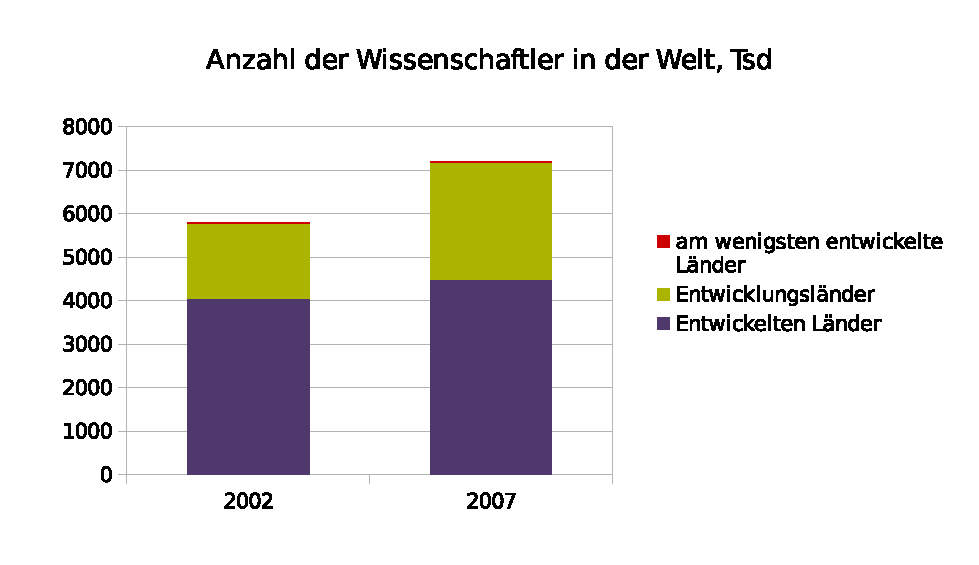
\includegraphics[width=0.8\textwidth]{fig1}
\caption{Zahl der Wissenschaftler weltweit, UNESCO 2010}
\label{fig:fig1}
\end{figure}
Andere Daten, welche die oben genannten Tendenzen bestätigen, beschreiben die Anzahl der Publikationen in der Welt. In 6 Jahre hat sich die Anzahl der Publikationen von 733.305 auf 986.099 erhöht, was ca. 34,5\% Wachstum entspricht. Der größte Anteil entfällt auf die entwickelten Länder, obwohl die Entwicklungsländer ein signifikantes 105,9\% Wachstum zeigen (Abbildung \ref{fig:fig2})\\
\begin{figure}[h!]
\centering
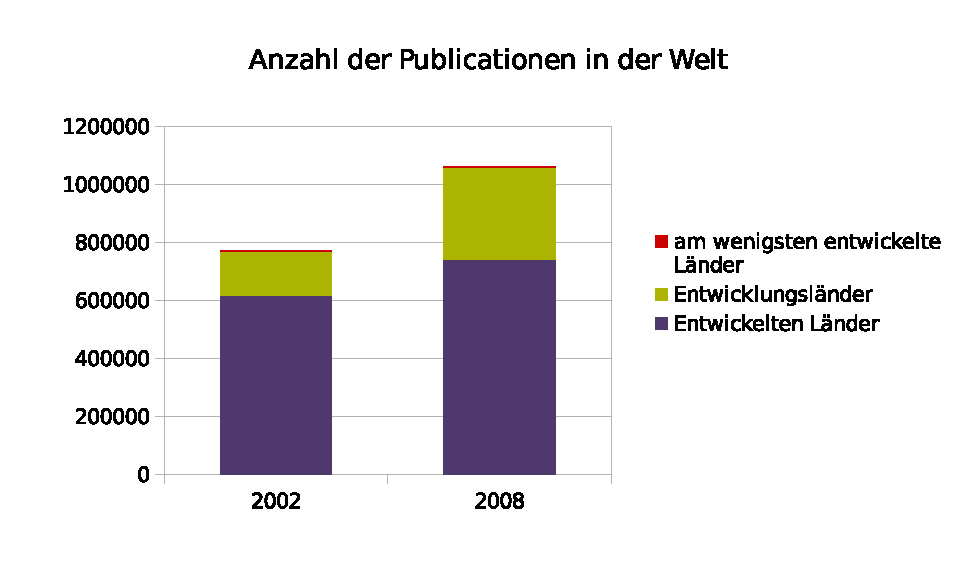
\includegraphics[width=0.8\textwidth]{fig2}
\caption{Anzahl der Publikationen in der Welt, UNESCO 2010}
\label{fig:fig2}
\end{figure}
Auf Grund dieser Daten, kann man feststellen, dass  wichtige Märkte sich in den entwickelten Ländern befinden. Die Entwicklungsländer zeigen jedoch riesige Wachstumspotenziale und werden deshlab nicht außer Acht gelassen. 
Zusammenfassend kann man sagen, dass der Markt potenzieller Kunden in den letzten Jahren ein gutes Wachstum verzeichnet hat und dabei sehr gute Aussichten auf weitere Entwicklung bestehen.

\subsection{Auswahl der regionalen Märkte}
Die Auswahl der regionalen Märkte ist ein wichtiger Teil der Marketingstrategie. Konzentration auf eine begrenzte Liste der regionalen Märkte lässt die regionalen Eigenschaften besser berücksichtigen, um möglichst die besten Dienstleistungen anzubieten. Enge Zusammenarbeit auf dem regionalen Markt und Partnerprogrammene sollten den Erfolg der Absatz unterstützen und neue Richtungen in der Entwicklung darstellen.\\
Um richtige regionale Märkte auszuwählen, werden nur die Länder ausgewählt, die die maximale Anzahl der Wissenschaftler haben, da die Wissenschaftler die Endnutzer von SemLit sind. \\
Die Auswahl der Länder erfolgt mit Hilfe der Angaben von UNESCO 2010 über die Anzahl der Wissenschaftler in jedem Land. Es werden nur die Länder ausgewählt, die zusammen ca. 70\% von der gesamten Anzahl aller Wissenschaftler in der Welt stellen. Die Zusammenfassung der Entwicklung der Anzahl der Wissenschaftler ist in Tabelle \ref{tab:ABC} dargestellt.\\
\begin{table}[h!]
  \centering
  \begin{large}
  \begin{tabular}{c}\hline
  \\
  {\color{orange}Neun ausgewählte Länder stellen}\\
  {\color{orange}ca. 70\% aller SemLit-Kunden weltweit.}\\
  \\\hline
  \end{tabular}
  \end{large}
\end{table}
Wie man aus Tabelle \ref{tab:ABC} sehen kann, machen neun ausgewählte Länder ca. 70\% aller Wissenschaftler in der Welt aus. Viele davon zeigen auch signifikante Wachstumsraten von mehr als 50\% in 5 Jahren. Dazu gehören China und Südkorea.


\begin{table}[h!]
  \centering
  \begin{footnotesize}
  \begin{tabular}{|l|r|r|r|r|r|}\hline
  \textbf{Land} & \multicolumn{4}{ c| }{\textbf{Anzahl der Wissenschaftler, Tsd.}} & \textbf{Wachstum}\\
  & 2002 & \% gesamt & 2007 & \% gesamt & \\ \hline
Welt & 5810.7 & 100.00\% & 7209.7 & 100.00\% & 24.08\% \\ \hline
Vereinigte Staaten & 1342.5 & 23.10\% & 1425.6 & 19.77\% & 6.19\% \\
China & 810.5 & 13.95\% & 1423.4 & 19.74\% & 75.62\% \\
Japan & 646.5 & 11.13\% & 710 & 9.85\% & 9.82\% \\
Russische Föderation & 491.9 & 8.47\% & 469.1 & 6.51\% & -4.64\% \\
Deutschland & 265.8 & 4.57\% & 290.9 & 4.03\% & 9.44\% \\
Vereinigtes Königreich & 198.2 & 3.41\% & 254.6 & 3.53\% & 28.46\% \\
Südkorea & 141.9 & 2.44\% & 221.9 & 3.08\% & 56.38\% \\
Frankreich & 186.4 & 3.21\% & 215.8 & 2.99\% & 15.77\% \\
Kanada & 116 & 2.00\% & 139 & 1.93\% & 19.83 \% \\ \hline
Alle ausgewählten Länder & 4199.7 & 72.28\% & 5150.3 & 71.44\% & 22.63\% \\ \hline
  \end{tabular}
  \end{footnotesize}
  \caption{Länder mit größtem Anteil der Wissenschaftler, basierend auf Daten von UNESCO 2010}
  \label{tab:ABC}
\end{table}


Für alle ausgewählten Länder werden andere wichtige Parameter geschätzt wie z.B. Bruttoinlandsausgaben für Forschung und Entwicklung (GERD) pro Wissenschaftler. Dieser Parameter zeigt, wie viel Geld in die Forschung und Entwicklung investiert wird. Je höher diese Zahl ist, desto höher ist die Wahrscheinlichkeit, dass Wissenschaftler das Geld nicht nur für reine Forschung, sonder auch für Dienstleistungen, die diese Forschung erleichtern könnten, zahlen werden. In Tabelle \ref{tab:ABC2} sind die Angaben zur Entwicklung der Bruttoinlandsausgaben für Forschung und Entwicklung pro Wissenschaftler präsentiert. Wie man aus Tabelle \ref{tab:ABC2} sehen kann, investieren entwickelte Länder sehr viel Geld in Forschung und Entwicklung, was als eine gute Chance für SemLit bewertet werden kann. 
\begin{table}[h!]
  \centering
  \begin{footnotesize}
  \begin{tabular}{|l|p{3cm}|p{3cm}|r|}\hline
  \textbf{Land} & \multicolumn{2}{ r| }{\textbf{GERD pro Wissenschaftler, \$ Tsd.}} & \textbf{Wachstum} \\
  & 2002 & 2007 & \\ \hline
Deutschland & 213.1& 248.4 & 16.56\% \\
Vereinigte Staaten & 206.4 & 243.9 & 18.17\% \\
Japan & 167.3 & 208.4 & 24.57\% \\
Frankreich & 204.7 & 196.1 & -4.20\% \\
Südkorea & 158.6 & 186.3 & 17.47\% \\
Kanada & 165 & 170.7 & 3.45\% \\
Vereinigtes Königreich & 154.6 & 152.2 & -1.55\% \\
China & 48.4 & 72 & 48.76\% \\
Russische Föderation & 32.4 & 50.1 & 54.63\% \\ \hline
  \end{tabular}
  \end{footnotesize}
  \caption{Bruttoinlandsausgaben für Forschung und Entwicklung (GERD) pro Wissenschaftler, basierend auf Daten von UNESCO 2010}
  \label{tab:ABC2}
\end{table} 



\subsection{Schätzung des Marktvolumens}
Schätzung des Marktvolumens ist für den Bereich Wissenschaft nicht einfach, da genauere Daten über die Anzahl und Budget nicht die Realität abbilden können. Deswegen werden diese Daten grob aus vorhandenen Daten abgeleitet. Zuerst wird die gesamt Anzahl der Wissenschaftler und Bruttoinlandsausgaben für Forschung und Entwdie Zahl der Publikationen in Bereich Ingenieurwesen und Technologie, die in diesen Ländern publiziert wurden. 
\begin{table}[h!]
  \centering
  \begin{large}
  \begin{tabular}{c}\hline
  \\
  {\color{orange}Verhältnis Zahl der Wissenschaftler}\\
  {\color{orange}zur Anzahl aller Publikationen ist ca. 7.}\\
  \\\hline
  \end{tabular}
  \end{large}
\end{table}
Aus resultierenden Daten über die Anzahl der Publikationen kann ein Verhältnis-Koeffizient berechnet werden, der eine grobe Schätzung über den Anteil von Ingenieurwesen und Technologie in der gesamten wissenschaftlichen Tätigkeit abgeben kann. Andere Koeffizienten, die wichtig sein könnten, sind Verhältnis von Anzahl der Wissenschaftler/Anzahl aller Publikationen sowie das Verhältnis von Bruttoinlandsausgaben für Forschung und Entwicklung/Anzahl der alle Publikationen. Dieser Koeffizienten zeigen, dass durchschnittlich 7 Wissenschaftler auf eine Publikation arbeiten und durchschnittliche Bruttoinlandsausgaben für eine Publikation ca. 1137,8 Tsd. von PPP\$ ist.
\begin{table}[h!]
  \centering
  \begin{footnotesize}
  \begin{tabular}{|l|l|}\hline
   \textbf{Parameter} &  \textbf{Wert} \\ \hline
  Anzahl der Wissenschaftler & 5150300 \\ \hline
  Bruttoinlandsausgaben für Forschung und Entwicklung & 865,5 Mrd. PPP\$ \\ \hline
  Anzahl der alle Publikationen & 760671 \\ \hline
  Anzahl der Publikationen im Ingenieurwesen & 101351
 \\
  und Technologie& \\ \hline
  Verhältnis (Publikationen in Ing.\& Tech. / alle Publikationen) & 13,3\% \\ \hline
  Verhältnis (Anzahl der Wissenschaftler / Anzahl der & ca. 7 \\
  alle Publikationen ) & \\ \hline
  Verhältnis (Bruttoinlandsausgaben für Forschung & 1137,8 Tsd. PPP\$\\
  und Entwicklung / Anzahl der alle Publikationen) & \\ \hline
  \end{tabular}
  \end{footnotesize}
  \caption{Angaben zu Märkten, basierend auf Daten von UNESCO 2010}
  \label{tab:ABC3}
\end{table}
 

\subsection{Wettbewerber}
Die wesentliche Wettbewerber im Feld der akademischen Suche sind Suchmaschinen. Normalweise bieten Suchmaschinen keine Zugang zum Volltext, sondern nur zum Abstract und den Referenzen. Wichtige Suchmaschine sind in Tabelle \ref{tab:wettSuch} zusammengefasst.
\begin{table}[h!]
  \centering
  \begin{footnotesize}
  \begin{tabular}{|l|l|l|l|}\hline
   \textbf{Name} &  \textbf{Suchverfahren} &  \textbf{Suchbereiche} &   \textbf{Zugang} \\ \hline
BASE - Bielefeld Academic  & Fast Search \& & Interdisziplinär & Kostenfrei \\
Search Engine & Transfer  & & \\ \hline
 Google Scholar & Eigene & Interdisziplinär & Kostenfrei\\\hline
 Microsoft Academic & Vertikale & Informatik & Kostenfrei \\
 Search & Suchmaschine & & \\ \hline
 CiteSeer & Eigene & Informatik & Kostenfrei \\ \hline
  \end{tabular}
    \end{footnotesize}
  \caption{Wichtige Suchmaschine}
  \label{tab:wettSuch}
\end{table} 
 
Zur zweiten Gruppe gehören Datenbanken. Sie stellen nicht nur die Suche in Abstracts und Referenzen bereit, sondern auch Zugang zur Volltexten. Normalweise sind die Suche und der Zugang zum Abstract kostenfrei. Um Zugang zum Volltext zu bekommen, muss das Abonnement zur Datenbank erworben werden. Wichtige Datenbanken sind in der Tabelle \ref{tab:wettDaten} gelistet. 
\begin{table}[h!]
  \centering
    \begin{footnotesize}
  \begin{tabular}{|l|l|l|l|}\hline
  \textbf{Name} &  \textbf{Suchbereiche} &  \textbf{Zugang} &  \textbf{Anbieter} \\ \hline
 SpringerLink & Interdisziplinar & Abonnement & Springer\\ \hline
 Academic Search & Interdisziplinar & Abonnement & EBSCO Publishing\\ \hline
 IEEE Xplore & Informatik \& & Abonnement & IEEE\\ 
 & Elektrotechnik & & \\ \hline
 Scopus & Interdisziplinar & Abonnement & Elsevier\\ \hline
 Web of Science & Interdisziplinar & Abonnement & Thomson ISI \\ \hline
  \end{tabular} 
    \end{footnotesize}
  \caption{Wichtige Datenbanken}
  \label{tab:wettDaten}
\end{table} 


\subsection{Alleinstellungsmerkmal und Kundennutzen}
Der wesentliche Unterschied zwischen SemLit und den bereits existierenden Angeboten auf dem Markt ist die semantische Suche und Verwaltung von Publikationen sowie der Self-Learning Algorithmus, um neue, relevante Publikationen zu finden. Auf der einen Seite stellt SemLit ein Dienstleistung bereit, ähnlich der von Suchmaschinen. Auf der anderen Seite gibt es eine Möglichkeit, auf bevorzugte Datenbanken und Quellen zuzugreifen.\\
SemLit ist sehr flexibel in der Benutzung. Wenn die Kunden bereits existierende Abonnements für eine der Datenbanken haben, kann SemLit als eine erweiterte Suchmaschine genutzt werden. D.h. Kunden können einen glatten Übergang von vorhandener Lösung zu SemLit durchführen oder SemLit als Erweiterung nutzen. 



\newpage

%%%%%%%%%%%%%%%%%%%%%%%%%
% Marketingstrategien Igor
%%%%%%%%%%%%%%%%%%%%%%%%%
\section{Marketingstrategien}



\subsection{Dienstleistungsformen}

Die Dienstleistung stellt Zugangsformen für Kunden dar:
\begin{itemize}
\item Webauftritt
\item App für Mobile Geräte
\item RSS Feed
\end{itemize}

Die Dienstleistung wird wird vor allem als Webauftritt dargestellt. App für Mobile Geräte und RSS Feed sind für Unterstützung der Webauftritt und Erweiterung der Nutzbarkeit und Nutzungserfahrung genutzt.\\

Die Dienstleitung stellt folgende Funktionen zur Verfügung:
\begin{itemize}
\item Sematische Suche der Publikationen
\item Suche in verwandte Felder. 
\item Verwaltung und Auswahl der wissenschaftlicher Suchquellen
\item Gestaltung von eigene Publikationslisten und Share-Funktion.
\item Gestaltung von Literaturverzeichnis für eigene Publikationen und Export-Funktionen in {\LaTeX} und andere Formaten. 
\item Verwaltung genutzter Publikationen
\item Self-Learning Algorithmus zur Verbesserung Suchergebnisse, basiert auf vorher gesuchte Publicationen.
\end{itemize}

Dieser Funktionen sind Anfangsfunktionen und werden durch Kunden-Feedback aktualisiert. 

\subsection{Nutzungsverfahren der Dienstleistung}
Die Dienstleistung für Endnutzer wird auf folgende Bedingungen angeboten:
\begin{itemize}
\item Funktion der Sematische Suche wird auf Webauftritt kostenlos und ohne Anmeldung angeboten
\item Zugang zur andere Funktionen der Dienstleistung erfolgt nur nach der Anmeldung und entsprechend der ausgewählte Nutzungsform. 
\end{itemize}
Dieser Gliederung dient für Kundengewinnung und stellt eine Möglichkeit die Dienstleistung unverbindlich zur nutzen. Die genaue Nutzungsformen werden in der Abschnitt Monetarisierung dargestellt. 

\subsection{Monetarisierung}

Die Monetarisierung wird von zwei Perspektiven Betrachten - direkt und indirekt. Bei direkte Monetarisierung, Geldeinfluss kommt gerade von Kunden. Die Kunden können die Dienstleistung in zwei Formen nutzen:
\begin{itemize}
\item \textbf{Microtransactions}. Kunden haben eine Möglichkeit nur für Abgefragte Information zu zahlen. 

\item \textbf{Abonnement}. Kunden zahlen feste Preis per Monate für Dienstleistungsnutzung, die in zwei Varianten gegliedert - Basic und Professional.
\end{itemize}

Microtransactions sind gut für private Kunden geeignet, die Information nicht ständig brauchen. Dieser Form erlaubt einmalige Nutzung der verfügbare Funktionen pro eine Zahlung. Abonnement ist gut für Wissenschaftliche Einrichtungen und Unternehmen geeignet. Man kann von zwei Zugangsniveau wählen. Basic stellt eine Möglichkeit kostengünstig Funktionen "Suche in verwandte Felder" und "Verwaltung und Auswahl der wissenschaftlicher Suchquellen" nutzen. Bei Professional, kann man alle existierende Funktionen unbegrenzt nutzen.\\

Bei indirekte Ansicht wird das Geldeinfluss aus Quellen, die nicht bei Endnutzer sind. Dieser Quellen sind
\begin{itemize}
\item \textbf{Sponsorships}. Geldeinfluss von Unternehmen oder Einrichtungen, die Bekanntheit zu erhöhen oder naher Kommunikation mit bestimmte Kundengruppe gestalten wollen.
\item \textbf{Werbung}. Kontext-basierte Werbung auf Webauftritt.
\end{itemize}

Zusammen direkte und indirekte Monetarisierung stellen eine Möglichkeit eine glatte Geldeinfluss zu gestalten und am schwierige Anfangsphase Finanziell gesichert sein.

 
\subsection{Kommunikationspolitik}

Für eine erfolgreiche Markteintritt und Absatz braucht man eine Kommunikationspolitik mit Kunden festzustellen und entsprechend nutzen. Um die Dienstleistung für potenzielle Kunden bekannt zumachen und eine Möglichkeit zu gestalten die Dienstleistung zu nutzen, werden folgende Maßnahmen durchgeführt: 
\begin{itemize}
\item Freemium: 3 Monate von kostenfreie Nutzung der Professional-Version für Kunden, die Basic-Version gekauft haben.
\item 3 Monate kostenlose Zugang zur Basic-Version, den bei Partnern ausgegeben wird (Webseiten, Zeitschriften etc.)
\item Speziale Angebote für wissenschaftliche Einrichtungen (Rabatte oder kostenlose Zugang)
\end{itemize}

\subsection{Markteintrittplan}

Markteintritt kann in vier Phasen gegliedert werden. Alle Phasen sollen Erfolg der Dienstleistung auf den Markt sichern und unterstützen: 
\begin{enumerate} 
\item Vorbereitung
\item Eintritt 
\item Kontrolle 
\item Anpassung 
\end{enumerate}

Wahrend der \textbf{Vorbereitung Phase} wird die Infrastruktur gebaut. Der Markteintritt soll mit schon funktionierte Dienstleistung erfolgen. Zu dieser Phase zahlt noch die Marketingvorbereitungsmaßnahmen. Dieser Phase befasst:
\begin{itemize}
\item Gestaltung der Suchmaschine
\item Anmeldung der Domain für Webauftritt
\item Gestaltung der Markenrichtlinien (Logo, Farben etc.)
\item Werbematerialvorbereitung
\item Gestaltung der Webauftritt, Mobile App und RSS Feed 
\item Testen der alle Funktionen 
\item Gestaltung der Infrastruktur (Büro, Miete der Rechnerkapazitäten oder Einkauf, Unternehmensrundung, Buchhaltung, Juristische Beratung etc.)
\end{itemize}

Nach der Vorbereitung wird \textbf{Markteintritt} durchgeführt. Dieser Phase ist schwierig und verlangt viel Konzentration und Aufwand. Es wird ausgeführt:
\begin{itemize}
\item Veröffentlichung der Webauftritt 
\item Start der Kommunikationspolitikmaßnahmen und Search Engine Optimization (SEO)
\end{itemize}

Mit Hilfe der \textbf{Kontrolle} kann man alle Parameter, die für Funktionieren der Dienstleistung wichtig sind, kontrollieren und entsprechende Maßnahmen durchzuführen. Man soll die Parameter so zu wählen, dass sie die Wirklichkeit spiegeln. Eine von Parameter könnte sein:
\begin{itemize}
\item Besucheranzahl von Webauftritt 
\item Anzahl der neue Anmeldungen 
\item Anzahl der Suchanfragen
\item Statistik an genutzte Datenquellen
\item Variablenkosten 
\end{itemize}

Zusammen mit der ständige Kontrolle sollte die \textbf{Anpassung} gemacht werden. Alle Maßnahmen soll gut angepasst werden, um maximale Erfolg und Verbesserung der Dienstleistung zu verfolgen.


\newpage

%%%%%%%%%%%%%%%%%%%%%%%%%
% Unternehmensplanung Igor
%%%%%%%%%%%%%%%%%%%%%%%%%
%
\section{Unternehmensplanung}


- geplante Rechtsform und Organisation bzw. Organigramm für das zu gründende Unternehmen

Der erste Mitarbeiter in Ihrem Unternehmen sind zunächst Sie selbst: Beschreiben Sie daher, welche beruflichen Erfahrungen Sie in der Branche gesammelt haben und wie Ihre bisherigen Erfolge aussahen. Haben Sie vielleicht eine Weiterbildung gemacht oder sich auf anderem Wege wertvolles Wissen angeeignet? Wie sieht Ihre Personalplanung für die nächsten drei bis fünf Jahre aus: Wollen Sie überhaupt Mitarbeiter einstellen und wenn ja, wie viele? Wollen Sie vielleicht mit freien Mitarbeitern oder Aushilfen zusammenarbeiten? So wie Sie Ihre eigenen Kenntnisse aufgelistet haben, sollten Sie auch die Qualifikationen Ihrer möglichen Partner und der schon feststehenden Mitarbeiter beschreiben.


%\newpage

%%%%%%%%%%%%%%%%%%%%%%%%%
% Chancen und Risiken Artem
%%%%%%%%%%%%%%%%%%%%%%%%%
\section{Chancen und Risiken}
In diesem Abschnitt diskutieren wir interne Faktoren und externe Umweltbedingungen, die sich positiv auf das Start-Up auswirken, beschreiben aber auch mögliche Risikofaktoren und zeigen, wie \textsc{SemLit} sie bewältigen kann.
\subsection{Stärken}
\textbf{Technologie}\\
Unsere größte Stärke liegt zweifelsohne in der innovativen semantischen Technologie. Dabei konnte sie sich schon in zahlreichen anwendungsorientierten Forschungsprojekten bewähren und hat auch gute Ergebnisse geliefert.
\\
\\
\textbf{Skalierbarkeit und Wachstum}\\
Die angewandte Technologie bringt wiederum den Vorteil mit sich, dass sie sehr gut skaliert und ohne großen Aufwand auf neue Wissens-Domänen angewandt werden kann. Damit hat SemLit das Potential, sich schnell und kostengünstig neuen Kundengruppen zuwenden zu können. So wäre es beispielsweise in naher Zukunft möglich, den Informationsmarkt für Rechts- und Finanzliteratur in den Fokus zu nehmen. Sowohl in dem einen, als auch im anderen Sektor kann man präzise eine Menge an hoch-qualitativen Online-Quellen für relevante Veröffentlichungen identifizieren und dazuschalten. Im Ergebnis wäre eine Kundengruppe mit besonders hoher Zahlungsbereitschaft gewonnen.
\\
\\
\textbf{Standort}\\
Bei der gegenwärtigen Lage in Sachen Datenschutz und -sicherheit ist ein Unternehmenssitz in Deutschland von großem Vorteil. Die hohen Standards hierzulande bilden ein überzeugendes Argument, besonders für Kunden aus dem angelsächsischen Raum und insbesondere angesichts neuester Datenschutzskandale.

\subsection{Schwächen}
\textbf{Recruiting im Start-Up-Unternehmen}\\
Als Start-Up ist es nicht einfach, die besten Mitarbeiter anzuwerben. Während die finanzielle Situation keine hohen Gehälter zulässt, stellt die Geschäftslage hohe Arbeitsbelastungen in Aussicht. Diesem Problem wollen wir mit einer wenig rigiden Arbeitszeitplanung und Aussicht auf Erfolgsbeteiligung entgegenwirken. 
\\
\\
\textbf{Kommerzielle Nutzung von Abstracts}\\
Eine weitere Frage erwächst aus der kommerziellen Nutzung von Abstract-Texten. Die Verlage veröffentlichen diese im Normalfall zur unentgeltlichen Nutzung. Ob bei massivem Crawling von Abstracts mit einer Rechtsklage zu rechnen ist, muss beim Rechtsexperten endgültig geklärt werden. \\
Eigentlich ist SemLit aus unserer Sicht letztendlich sogar vorteilhaft für die Verlage, weil es zu weitreichender und einfacher Verbreitung ihrer Publikationen führt.

\subsection{Chancen}
\textbf{Positive Marktstimmung}\\
Der Markt ist bereit für semantische Technologien: Der Gartner-Bericht 2013\footnote[5]{Quelle: http://www.gartner.com/newsroom/id/2359715} erkennt in semantischen Technologien den Schlüssel zur Bewältigung kommender Herausforderungen in der Informationsverarbeitung. Nach unserer Einschätzung gehen damit positive Kunden-Erwartungen, eine geringere Hemmschwelle und auch höhere Zahlungsbereitschaft einher.
\\
\\
\textbf{Exit durch Übernahme}\\
Als stark spezialisiertes Unternehmen in einem hochinnovativen Technologiesegment ist SemLit ein guter Kandidat für die Übernahme durch einen der großen Spieler. Außerdem werden die Vorzeichen einer Übernahme durch die kommende Erholung der Weltkonjunktur begünstigt. Für SemLit ist das die bevorzugte Exit-Strategie.

\subsection{Risiken}
\textbf{Konkurrenz}\\
Der beste Kandidat für einen direkten Konkurrenten wäre Google. Neben massiver techno-logischer und personeller Kompetenz verfügt Google mit dem Dienst Scholar bereits über die nötige Datengrundlage.\\
Bis jetzt deutet allerdings nichts darauf hin, dass Google Scholar zu einem vergleichbar umfassenden und spezialisierten Angebot ausgebaut werden soll. 
\\
\\
\textbf{Micropayment-Gebühren}\\
Um die Reichweite im Markt zu erhöhen, wird SemLit auf einen Micropayment-Dienstlesiter wie PayPal angewiesen sein. Bei jeder Transaktion würden deshalb entsprechende Gebühren anfallen. Außerdem könnte sich mit der Zeit ihre Höhe ändern.\\
Derzeit verlangt PayPal jedoch einen vertretbaren Aufschlag: Für Zahlungen innerhalb Deutschlands entstehen ca. 2,5\% und international etwa 3-5\% an Umsatzgebühren. Damit ist die stark erhöhte Reichweite bei diesem Stand relativ billig erkauft.

\newpage

%%%%%%%%%%%%%%%%%%%%%%%%%
% Finanzplanung Artem
%%%%%%%%%%%%%%%%%%%%%%%%%

\section{Finanzplanung}
- Einnahmen- und Ausgabenplanung für die ersten zwei Jahre nach Gründung mit Erläuterungen 

Geld spielt bei der Existenzgründung eine große Rolle. Daher sollten Sie in Ihrem Businessplan diesen Punkt exakt ausarbeiten und mit Zahlen und Fakten belegen. In Teil 1 nennen Sie die geplanten Investitionen, die Sie am Anfang und im Laufe der ersten Zeit tätigen. Listen Sie alle größeren Anschaffungen der nächsten drei bis fünf Jahre auf. Aus dieser Liste ergeben sich der Kapitalbedarf und die jährlichen Abschreibungen. Teil 2 ist der Liquiditätsplan: Er zeigt alle Ausgaben und Einnahmen, die Sie in den nächsten Jahren erwarten. Für das erste Jahr machen Sie eine monatliche Aufstellung, für die Folgejahre reicht eine Auflistung zunächst nach Quartalen, später pro Halbjahr. Darüber hinaus erstellen Sie eine Gewinn- und Verlustrechnung über den voraussichtlichen Geschäftsverlauf samt Umsätzen, Ausgaben und Gewinnen. Anschließend ordnen Sie die Finanzierungsposten den Kapitalgebern zu: Wie viel Eigenkapital haben Sie, und wofür setzen Sie es ein? Und wie viel Unterstützung durch Banken oder andere Kreditgeber brauchen Sie für welche Posten? Vergessen Sie auch nicht eine Reserve für unvorhersehbare Ausgaben.



\newpage




\end{document}